\documentclass[12pt]{article}
\usepackage{fontspec}
\usepackage{graphicx}
 
\setmainfont{Times New Roman}
\title{\textit{\textit{BreakHis}} images classification with \textit{CNN}}
\author{Maciej Dzikowski}
\date{\today}
   
\begin{document}
\maketitle
     
\begin{abstract}
The constant and unstoppable evolution of new machine learning technologies leads to the co-development of every domain, which produces a large amount of data. One of the most promising fields in this respect is medicine, especially oncology. The variety of tumors results in receiving different datasets for every examined type, which are widely analysed, and then the results are often published. One of such papers is \textit{Cancer diagnosis in histopathological image: CNN based approach}\cite{1} which has been reproduced as a goal of this project.

The main objective of the project was to create a convolutional neural network which will allow for classifying cancer by its malignancy. The data used was \textit{BreakHis} dataset\cite{2} containing histopathological stained images. The photos were used for training the obtained model and comparing evaluation results with publication.

In an attempt to improve the architecture, an autoencoder based on the previous model was implemented.
\end{abstract}



\section{Introduction}
Nowadays, we can observe a great interest in machine learning. In every area of life, in any field of interest, we are bombarded with news or advertisements with popular terms like artificial intelligence, neural networks or deepfake that more or less reflect the essence of the machine learning methods. The trend can also be observed in the scientific community. The growing necessity for large amounts of data analysis from almost all fields of science makes it necessary to use the latest techniques. One of the most promising areas is medicine, especially oncology which produces the greatest amount of information. The reason for this is the wide variety of tumor types, their causes and treatments.


\subsection{Breast Cancer}
Breast cancer is the most common malignant tumor diagnosed in women in Poland - nearly $22\%$ of all recognized. Every year more than $18$ thousand cases have been reported, and it is estimated that within ten years, the value will reach $20$ thousand. In 2017, the incidence rate for women was $53$ per $100$ thousand, and the mortality rate equals $14.95$ per $100$ thousand\cite{3}.

In United States of America, breast cancer is also the most common diagnosed tumor in women and accounts for $30\%$ of all cases\cite{4}.
For both countries, it has the second highest mortality rate after lung and bronchus cancer. Women between the ages of 50 and 69 are most often affected by this type of a cancer. In men it is rare and stands for only about $1\%$ of all diagnosed breast cancer cases\cite{3}.


\subsection{Diagnostics}
\subsubsection{Prevention\cite{3}}
Early diagnosis and prevention is very important for every tumor type, especially breast cancer due to the high risk of death. The earlier a treatment procedure will be implemented, the better the outcome will be. For example, in Poland the five-year survival rate between 2000 and 2014 increased by more than $5$ percentage points.

The most significant risk factors for breast cancer are age, reproductive factors, unhealthy lifestyle, exposure to ionizing radiation, and family history of cancer.

The prevention can be divided into primary and secondary prevention. Primary prevention includes: a healthy body weight, physical activity, reducing alcohol consumption, avoiding smoking, and limiting the use of hormone replacement therapy. Secondary prevention includes all tests, medical examinations recommended in the case of being in a risk group. It can be carried out without indications as part of a screening program or during a non-routine visit to the doctor. The approaches the doctor can use: physical exam, laboratory tests, imaging tests or biopsy.


\subsubsection{Methods}
During the psychical exam, a doctor can look for indicators which may indicate the presence of cancer like skin colour changes, organ enlargements or lumps. In case of breast cancer, it is recommended to perform self-exam (preferably every month) because lumps are the most common symptom\cite{3}.

Laboratory tests can help to identify deviations from the norm caused by a tumor. Blood or urine tests are not used to diagnose breast cancer.

Imaging tests are a noninvasive way of examining organs. There are plenty of different methods, each with its benefits and drawbacks. Among them, some techniques used for breast cancer can be distinguished: computed tomography, mammography, magnetic resonance imaging, positron emission computed tomography, single-photon emission computed tomography, and ultrasonography\cite{5}.

The previously mentioned methods are not always entirely accurate hence there is a need to perform more invasive procedure - biopsy. During the process, a sample of cells from the suspicious area is collected. It can be colored by some staining element (usually hematoxylin and eosin) which will improve readability. Then, pathologists can examine the obtained sample under microscope or take pictures of it for future manual or computer-aided analysis\cite{1}.


\subsection{Deep Learning}
Lately, mathematical and statistical instruments known more widely as machine learning have become popular in science as well as in commercial projects. This is a result of the high performance of this techniques in many fields connected with data analysis like image or natural language processing, spam, detection, text mining or content recommendation\cite{6}.

Among these tools, deep learning is the most promising and is now experiencing its second youth. The most modern models focus on building and using neural networks, which are characterized by deep stacks of computations called layers. The layers are used to progressively extract features from the raw input. Such a neural networks are called deep neural networks\cite{6}.

The most fundamental part of the neural network is neuron, also called linear unit due to its formula ($y = wx + b$), which is simply an equation of the line. Every neuron has an input ($x$) with its weight ($w$) and a bias value ($b$) which allows to modify the output ($y$) independently of the input\cite{7}.

In the Figure \ref{fig:ANN} there is a schema of neural network with input layer, one dense layer (called also hidden since its output is never revealed)  and an output layer\cite{7}.

\begin{figure}
\centering
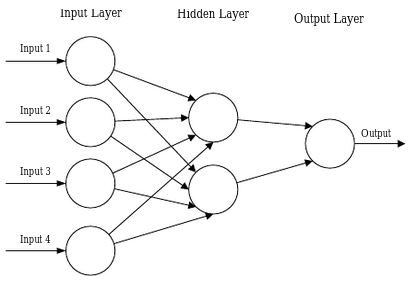
\includegraphics[width=0.7\textwidth]{ANN.png}
\caption{\label{fig:ANN}Schema of a three layer neural network\cite{7}.}
\end{figure}

It seems every neural network layer performs relatively simple transformation, and it is just too simple approach to achieve any significant output for complicated problems. However, with every layer added the network becomes more complex and thoughtfully designed and well-trained model can provide unexpectedly good results. Also, to improve the performance of the model, the activation functions are used to modify the neurons outputs. The most frequent used activation function is rectifier function (ReLU) which transforms every neuron in the layer result by returning $0$ for every negative value and leaving positive ones without changing\cite{8}.


\subsubsection{Convolutional Neural Networks} 
A convolutional neural network is a type of artificial neural network that is most often applied to image or natural language processing problems. Its uniqueness lies in the fact that, unlike the usual neural network, every neuron in a layer is not connected to all neurons in previous layer but only to the closest one. What is more, all the neurons in every layer have the same weight value.

The simplification in connections lets the model upholds the spatial aspect of the dataset used as an input. It means the convolutional neural network does not think that specific element of the input is all over it.

The convolutional neural network can have five types of layers (Figure \ref{fig:CNN}):
\begin{itemize}
\item Input layer - stores arrays of images pixels.
\item Convolutional layer - places a fitter over an array of image pixels using (or not specified activation function), what creates a convolved feature map.
\item Pooling layer - performs downsampling onto given input, what reduces the number of parameters.
\item Fully-connected layer - allows to perform a classification on the dataset.
\end{itemize}

\begin{figure}[!ht]
\centering
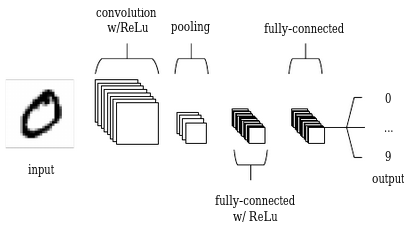
\includegraphics[width=0.7\textwidth]{CNN.png}
\caption{\label{fig:CNN}Schema of a four layer convolutional neural network\cite{7}.}
\end{figure}



\section{Materials and methods}
\subsection{Database}
Just like the authors of the publication\cite{1}, the data for the project was taken from the \textit{BreakHis} database\cite{2}. The dataset contain 7909 breast cancer histopathology images acquired with the same procedure (surgical open biopsy) from 82 patients.

The photos in the database are divided by procedure of receiving, tumor type, image magnification and tumor malignancy. The division into benign and malignant allows to perform supervised machine learning methods over the database. However, the more fragmented the data is, the more difficult is data wrangling process which has to be carried out before setting any model. Fortunately, along with the images has been provided a CSV format file with local paths to every file in the database, what made the process of reading data easier.

In the dataset there are 2480 images of benign and 5429 of malignant tumor (Figure \ref{fig:malignancy}). The quantitative advantage for malignant tumor is probably due to more frequent visits of patients in advanced stages of the disease.

\begin{figure}[!ht]
\centering
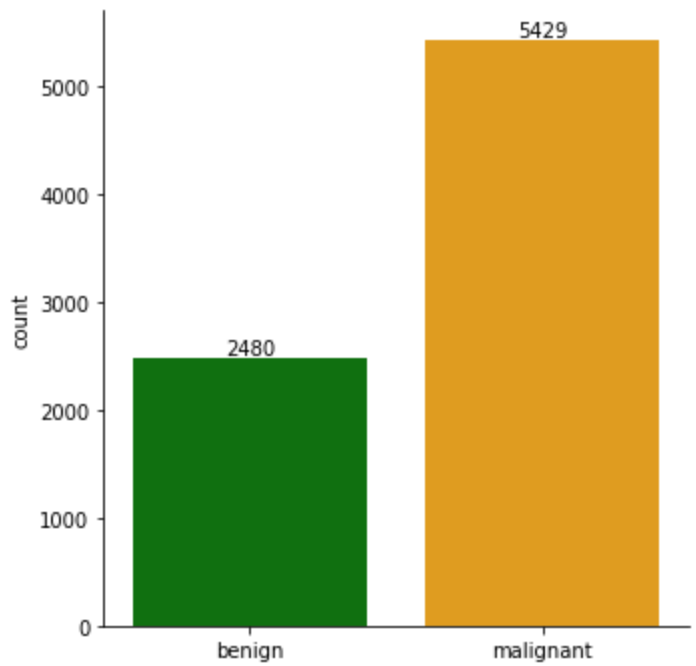
\includegraphics[width=0.5\textwidth]{malignancy.png}
\caption{\label{fig:malignancy}Distribution of images in dataset by malignancy.}
\end{figure}

The subsets resulting from partitioning by image magnification are almost of equal size and the ratio of benign to malignant images is similar (Figure  \ref{fig:magnification}).

\begin{figure}[!ht]
\centering
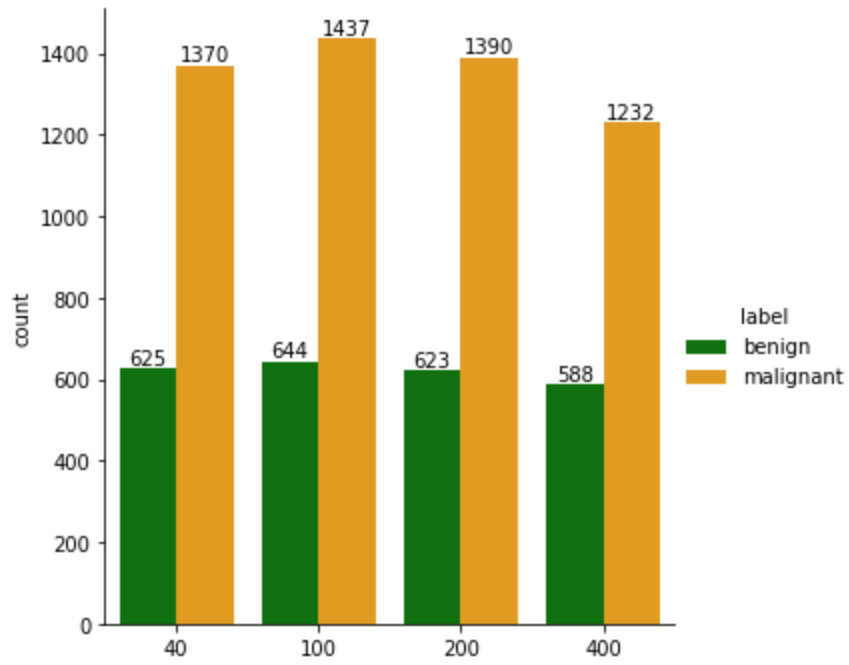
\includegraphics[width=0.6\textwidth]{magnification.png}
\caption{\label{fig:magnification}Distribution of images in dataset by magnification and malignancy.}
\end{figure}

All the above values are equal to results published in the publication\cite{1}. 

In Figure \ref{fig:sample}, there is a sample of images obtained from the database with labels.

\begin{figure}[!ht]
\centering
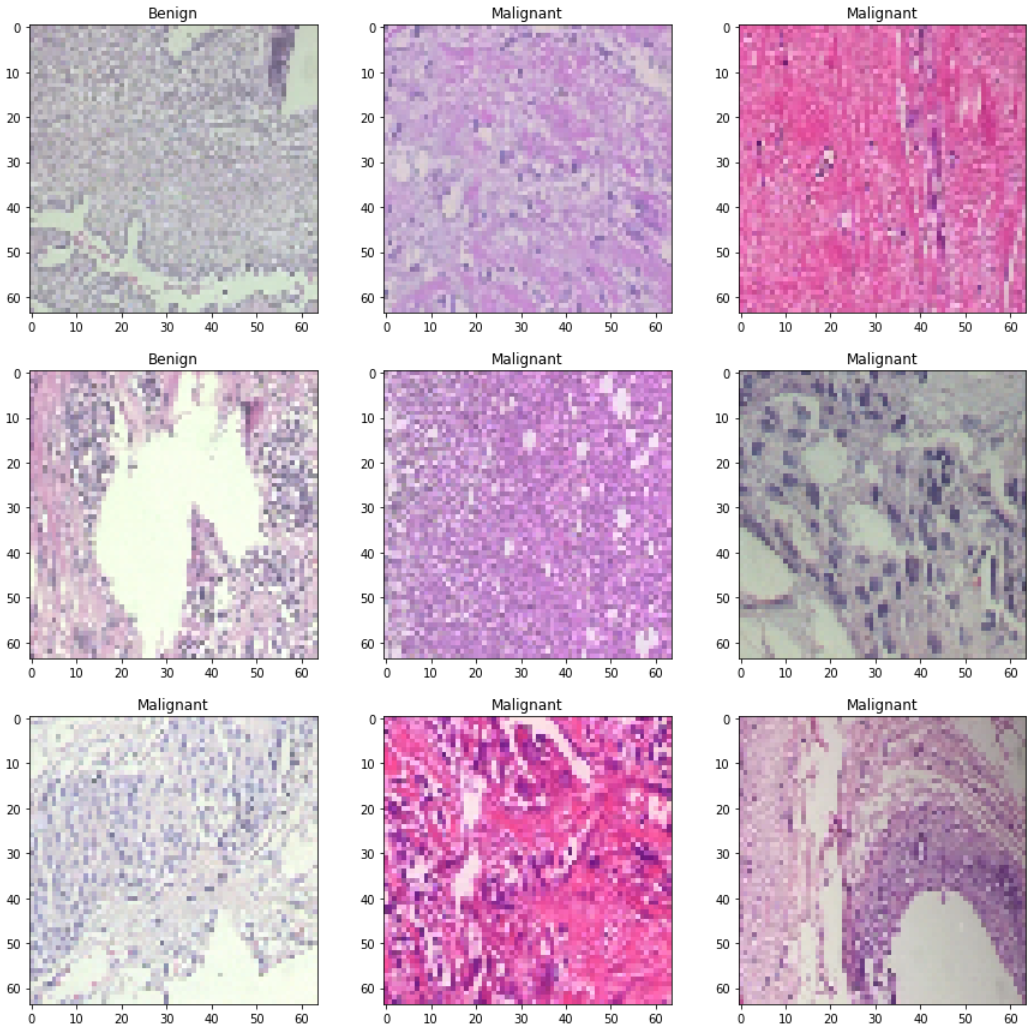
\includegraphics[width=0.9\textwidth]{sample.png}
\caption{\label{fig:sample}A sample of images with labels.}
\end{figure}


\subsection{Tools}
The entire project was made using \textit{Python} version 3.7.13 and \textit{Google Colaboratory}. All the plots were obtained with \textit{seaborn} 0.11.2 and \textit{Matplolib} 3.4.0 libraries. The data wrangling process was achieved with \textit{pandas} 1.3.5 library. The convolutional neural network model was build using \textit{TensorFlow} 2.8.2 library and its framework - \textit{Keras} 2.8.0. Its evaluation was made with \textit{scikit-learn} library.



\section{Results}
\subsection{Model}
In accordance with the assumption of the project, the same model had to be created. It was possible thanks to the exact specification presented in the publication\cite{1}, and in the Figure \ref{fig:model_sum} there is the obtained model summary.

\begin{figure}[!ht]
\centering
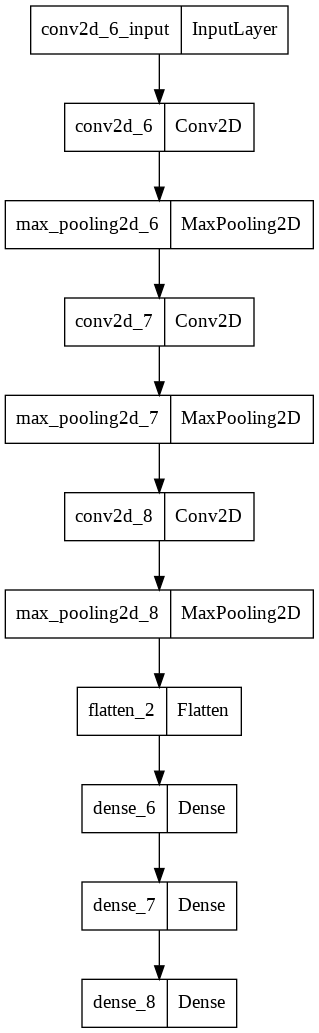
\includegraphics[width=0.32\textwidth]{model_sum.png}
\caption{\label{fig:model_sum}Summary of the received deep neural network model.}
\end{figure}

The convolutional neural network consists of three convolutional layers interspersed with three pooling layers. A stride size of all the layers is equal $1 x 1$. The filters numbers in the convolutional layers are $32$, $64$, $128$, respectively. The kernel size match $5 x 5$, and ReLU is an activation function for each. The pooling size of all the pooling layers is equal $3 x 3$.

To classify the images with the model, it was necessary to take the flattened weighted feature map from the convolutional neural network output and use it as an output to fully connected network. The network consists of three dense layers - two with $64$ filters and ReLU as an activation function, and the last with $2$ filters and softmax activation function.


\subsection{Evaluation}
The model fitting have been run with early stopping method to avoid overfitting of the model and save time by reducing number of epochs. The process took $17$ epochs, and the final loss and accuracy values were $40.54\%$, $84.20\%$ respectively. 

The obtained accuracy was worse than the accuracy shown in the publication ($93.45\%$)\cite{1}. Also, it was not achievable, due to technical reasons, to fit model on full dataset for $500$ epochs like in the paper. To achieve the same number of epochs, there appeared an idea to reduce dataset size, but despite reducing to 10\% and 1\%, the required fitting time remained the same.

Values received out of a classification report (Table~\ref{tab:report}) varied great from the shown in the publication\cite{1}. 

\begin{table}[!ht]
\centering
\begin{tabular}{l|r r r}
 & Precision & Recall & F1-score \\
\hline
Benign & 0.33 & 0.27 & 0.30 \\
Malignant & 0.68 & 0.74 & 0.71 \\
Avg/total & 0.51 & 0.51 & 0.51 \\
\end{tabular}
\caption{\label{tab:report}Classification report with summary of result.}
\end{table}

The same was the case with the confusion matrix (Figure \ref{fig:matrix}). The true positive and true negative values were similar and much higher than that the false positive and false negative values which were also similar to each other.
\clearpage

\begin{figure}[!ht]
\centering
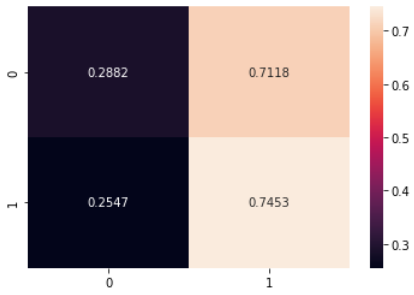
\includegraphics[width=0.7\textwidth]{matrix.png}
\caption{\label{fig:matrix}Confusion matrix. $0$ - benign, $1$ - malignant.}
\end{figure}

The percentage of correctly classified images in both groups (benign and malignant) as similar and amounted to slightly over 50\% (Figure \ref{fig:corr_class}).

\begin{figure}[!ht]
\centering
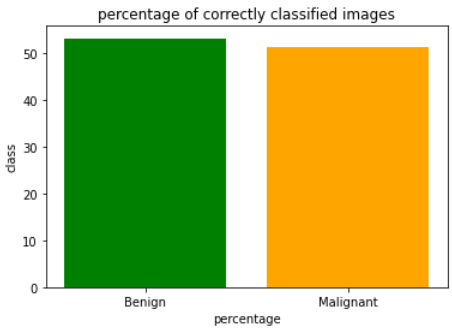
\includegraphics[width=0.7\textwidth]{corr_class.png}
\caption{\label{fig:corr_class}Percentage of correctly classified images in benign and malignant groups.}
\end{figure}


\subsection{Autoencoder}
Due to the unsatisfactory results and the suspicion that the reason may be different magnification of photos in the data set, an autoencoder has been added to the model. The autoencoder would have reduced the impact of the magnification.

The autoencoder consists encoder and decoder. The encoder was basically the previous convolutional + fully connected neural network model. The decoder above all had to accept flattened input and reshape it. So, it consists of input, dense, reshape layer, and five convolutional layers with one upsampling layer.(Figure \ref{fig:decoder_sum}. All of the convolutional layers has stride size equal $1 x 1$, and the filters numbers are 128, 64, 32, 32, 3, respectively. ReLu was an activation function for all layers except the last one where the softmax function is used.

\begin{figure}[!ht]
\centering
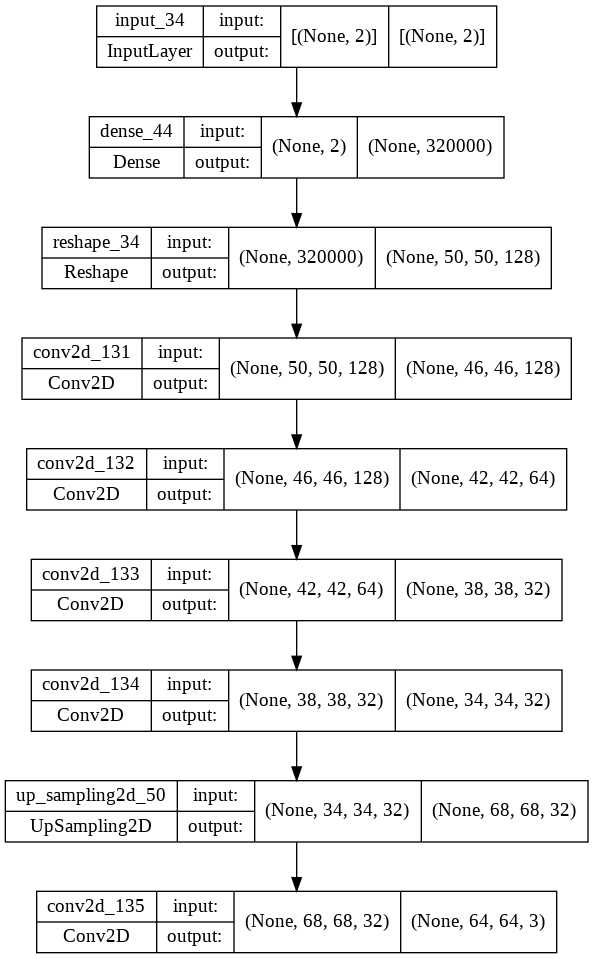
\includegraphics[width=0.52\textwidth]{decoder_sum.png}
\caption{\label{fig:decoder_sum}Schema of a decoder architecture.}
\end{figure}

The encoder and the decoder were merged into an autoencoder. An optimizer used to compile the model was Adam algorithm, and the loss function was categorical crossentropy. 

Unfortunately, the model could not be fitted and evaluated properly. More information is included in Jupyter Notebook file with the code.



\section{Discussion}
As shown in result section, the author's results were much more better (Table~\ref{tab:report_pub}) than obtained (Table~\ref{tab:report}) in this project.

\begin{table}[!ht]
\centering
\begin{tabular}{l|r r r}
 & Precision & Recall & F1-score \\
\hline
Benign & 0.91 & 0.88 & 0.89 \\
Malignant & 0.95 & 0.96 & 0.95 \\
Avg/total & 0.93 & 0.93 & 0.93 \\
\end{tabular}
\caption{\label{tab:report_pub}Summary of result from the publication\cite{1}.}
\end{table}

Also, the values received in confusion matrix are worse (Figure \ref{fig:matrix}) than in Figure \ref{fig:matrix_pub}, and do not indicate correct operation of the prepared model. The true positive and true negative values are similar what suggest that model more likely predicts malignant tumor. However, comparison by percentage of correctly classified images (Figure \ref{fig:corr_class}) seems to show something else - for both groups the right prediction is slightly above 50\%. Such a behaviour is possible in the encountered situation when the groups are not equal (Figure \ref{fig:malignancy}). The false positive and the false negative values are also similar what confirms the very poor performance of the model.
\clearpage

\begin{figure}[!ht]
\centering
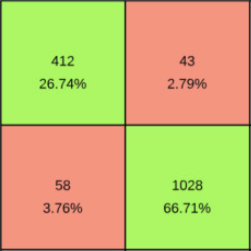
\includegraphics[width=0.5\textwidth]{matrix_pub.png}
\caption{\label{fig:matrix_pub}Confusion matrix from the publication\cite{1}. $0$ - benign, $1$ - malignant.}
\end{figure}

The main suspected reason for the unfavorable result was a mentioned several times difference in images magnification in the dataset. However, in spite of the attempts, it was not possible to find a working way to improve model performance.



\bibliographystyle{naturemag}
\bibliography{references}

\end{document}